\documentclass[11pt]{article}

% ---- layout and fonts
\usepackage[margin=1in]{geometry}
\usepackage[T1]{fontenc}
\usepackage[utf8]{inputenc}
\usepackage{lmodern}
\usepackage{microtype}
\usepackage{setspace}
\onehalfspacing

% ---- content
\usepackage{amsmath,amssymb}
\usepackage{graphicx}
\usepackage{longtable,booktabs,array,calc}
\usepackage{xcolor}
\usepackage[numbers,sort&compress]{natbib}
\usepackage{authblk}
\usepackage[colorlinks=true,linkcolor=blue!60!black,citecolor=blue!60!black,urlcolor=blue!60!black]{hyperref}

% allow common Unicode symbols in the text with pdfLaTeX (Overleaf default)
\usepackage{newunicodechar}
\newunicodechar{±}{\ensuremath{\pm}}
\newunicodechar{×}{\ensuremath{\times}}
\newunicodechar{≥}{\ensuremath{\geq}}
\newunicodechar{≤}{\ensuremath{\leq}}
\newunicodechar{≈}{\ensuremath{\approx}}
\newunicodechar{−}{\ensuremath{-}}
\newunicodechar{→}{\ensuremath{\rightarrow}}
\newunicodechar{λ}{\ensuremath{\lambda}}
\newunicodechar{μ}{\ensuremath{\mu}}
\newunicodechar{σ}{\ensuremath{\sigma}}
\newunicodechar{δ}{\ensuremath{\delta}}

% pandoc-generated lists and tables use these
\providecommand{\tightlist}{\setlength{\itemsep}{0pt}\setlength{\parskip}{0pt}}
\newlength{\cslhangindent}

% editing notes: \todo{...} shows in red; remove before submission
\newcommand{\todo}[1]{\textcolor{red}{[#1]}}

\title{inferCNV: inferring copy number alterations from single-cell transcriptomes}

\author[1]{Christophe Georgescu}
\author[1]{Timothy Tickle}
\author[1]{Maxwell Brown}
\author[1]{Yu Zhong}
\author[3]{Simon Kasif}
\author[1]{Aviv Regev}
\author[2]{Itay Tirosh}
\author[1]{Brian J. Haas}
\affil[1]{Broad Institute of MIT and Harvard, Cambridge, MA, USA \todo{confirm}}
\affil[2]{Weizmann Institute of Science, Rehovot, Israel \todo{confirm}}
\affil[3]{Boston University, Boston, MA, USA \todo{confirm}}
\date{Draft, \today}

\begin{document}
\maketitle

\begin{abstract}
Large-scale copy number alterations (CNAs) can be inferred from single-cell RNA-seq (scRNA-seq) data, which makes it possible to distinguish malignant from non-malignant cells and to define genetic subclones in the same data used to study cell states. The approach was introduced in single-cell studies of glioblastoma and was used in a series of subsequent tumour atlases. inferCNV is an R/Bioconductor package that implements and extends it, and it has been widely used since 2018. inferCNV compares the expression of genes ordered along the genome in tumour cells with that of a user-defined set of normal reference cells. It produces reference-normalised, positionally smoothed residual expression profiles; groups cells into subclusters; predicts discrete copy number states with a six-state hidden Markov model calibrated by in-silico spike-in simulation; and filters predicted CNAs with a Bayesian mixture model. Here we describe the algorithm and its reference implementation and illustrate its behaviour on simulated data and on tumours with DNA-based copy number measurements. Because CNAs are inferred relative to the reference cells, we show how the choice of reference shapes the results: on healthy blood cells and normal tissue sections, false calls followed cell-type expression programmes that the reference did not cover, could be predicted from expression alone, and fell several-fold when the reference included the lineage of the cells analysed. We also show that it applies without change to long-read single-cell and spatial data: on cancer cell lines profiled with PacBio Kinnex, ONT and Illumina sequencing, its calls agreed with cell-line copy number to a similar degree for all three platforms, and on Kinnex Visium HD sections it mapped tumour subclones in tissue. inferCNV is available from Bioconductor, GitHub and Docker Hub.

\end{abstract}

\section{Introduction}\label{sec:introduction}

Somatic copy number alterations (CNAs), ranging from focal amplifications to gains and losses of whole chromosome arms, are among the most frequent genetic changes in cancer, and some are characteristic of particular tumour types. Examples are the co-deletion of chromosome arms 1p and 19q in oligodendroglioma and the gain of chromosome 7 with loss of chromosome 10 in glioblastoma \citep{tirosh2016oligo, patel2014}. Copy number is usually measured from bulk DNA, which averages over all cells in a sample. Measuring it in single cells adds two kinds of information. First, it identifies the malignant cells of a tumour, which is not always possible from expression alone, because malignant cells can closely resemble their non-malignant counterparts. Second, it resolves genetic subclones and relates them to the transcriptional states and microenvironment of the same cells.

CNAs were first inferred from single-cell transcriptomes in a study of primary glioblastoma \citep{patel2014}. A gain or loss of a large genomic region shifts the expression of many neighbouring genes in the same direction. The expression of any single gene reflects its copy number only weakly, but the average over many genes ordered along a chromosome reveals the change. In that study, log-transformed expression values were centred on each gene's mean, averaged in a moving window of 100 genes along the genome, and centred again within each cell. No normal reference cells had been isolated; the few normal cells in the data were recognised because their profiles clustered with an averaged profile of bulk normal brain. Their mean profile then served as the baseline, against which the malignant cells showed the gain of chromosome 7 and loss of chromosome 10 typical of glioblastoma. Applied to cancer cell lines with both RNA-seq and SNP array data, the same smoothing gave profiles that correlated with array-based copy number (r = 0.72) \citep{patel2014}.

The approach, implemented by Itay Tirosh in MATLAB, was refined in a series of single-cell tumour studies. In oligodendroglioma, relative expression values were capped at $\pm$3 before smoothing so that single genes could not dominate a window. Separate baselines were also defined for each normal cell type, and a value was counted as altered only if it lay outside the range of those baselines by more than a small margin \citep{tirosh2016oligo}. Studies of IDH-mutant glioma and head and neck cancer then classified cells as malignant by two scores: the overall magnitude of a cell's CNA profile, and its correlation with the average profile of the tumour \citep{venteicher2017, puram2017}. A later glioblastoma study defined subclones from chromosome arms with bimodal CNA values \citep{neftel2019}. The method was used to identify malignant cells in further studies of melanoma \citep{tirosh2016melanoma} and H3K27M-mutant glioma \citep{filbin2018}. It was later released as the R package infercna \citep{laffy_infercna} and used to verify malignant cells in a pan-cancer atlas \citep{gavish2023}.

As single-cell profiling of tumours spread, there was a need for an open-source tool with which any group could apply the method routinely. We developed inferCNV for this purpose, as an R package based on Tirosh's method, and distributed it through GitHub and later Bioconductor \citep{tickle2019infercnv, infercnvBioc}. inferCNV kept the core of the original procedure: the log-transformed, depth-normalised expression, the cap on relative values, smoothing over a window of about 100 genes, per-cell centring, and subtraction bounded by the range of several normal reference groups. It began as a visualisation tool, from which CNAs were read by inspecting heatmaps. It was then extended to predict discrete copy number states with a hidden Markov model (HMM), building on the HMM of HoneyBADGER \citep{fan2018}. The HMM's states are calibrated by simulating spiked-in CNAs that match the depth and noise of each data set \citep{haas2021thesis}. inferCNV also assesses its calls with a Bayesian mixture model and partitions cells into CNA-based subclusters. It does not, however, include the score-based classification of malignant cells used in the original studies.

inferCNV has since been applied to many tumour types and platforms. Early uses that named the package were in melanoma \citep{jerbyarnon2018} and synovial sarcoma \citep{jerbyarnon2021}. It has been used with data from Smart-seq2 \citep{maynard2020}, droplet-based 10x Genomics \citep{ma2019, bi2021, steen2021}, Seq-Well \citep{raghavan2021} and single-nucleus RNA-seq \citep{slyper2020, terekhanova2023}. Applications include studies of uveal melanoma with single-cell DNA validation \citep{durante2020}, high-grade serous ovarian cancer \citep{izar2020}, breast cancer \citep{wu2021breast} and small cell lung cancer \citep{chan2021}, and a pan-cancer analysis of recurrent cell states \citep{barkley2022}. A full-text search of Europe PMC on 20 October 2026 found 2,741 articles that mention ``inferCNV'', rising from 3 published in 2018 to 758 in 2025. These are mentions in titles, abstracts or full texts rather than citations, and an undercount, because full text can be searched only for the articles that Europe PMC holds in full. The method has also been carried into spatial transcriptomics. SpatialInferCNV applies inferCNV to spatially barcoded spots to reconstruct clonal CNAs in situ, including in histologically benign tissue \citep{erickson2022}, and has been used by others \citep{pei2025}. inferCNV has also been applied directly to spot-based data \citep{wu2021liver, denisenko2024, lucas2024, mo2024, harwood2024} and to spatially barcoded single-nucleus data \citep{russell2024}.

Several other methods infer CNAs from single-cell transcriptomes; the main differences between them are the use of a normal reference and of allelic information. Among methods that use expression alone, some require no reference. CONICSmat fits mixture models to the expression of each chromosome arm \citep{muller2018conics}. CopyKAT identifies diploid cells itself and segments the genome of each cell \citep{gao2021copykat}. SCEVAN classifies cells and segments clonal profiles \citep{defalco2023}. sciCNV \citep{mahdipourshirayeh2022scicnv} and the Python reimplementation infercnvpy \citep{sturm_infercnvpy} produce continuous profiles. Allele-aware methods add the allelic imbalance of heterozygous variants in the reads, which can show loss of heterozygosity even when expression is unchanged. HoneyBADGER combines an expression HMM with an allele model \citep{fan2018}, and CaSpER uses allele shifts to refine expression signals at several scales \citep{serinharmanci2020}. Numbat phases variants with a population haplotype panel and infers a phylogeny of subclones \citep{gao2023numbat}, and XClone infers states separately from read depth and from phased allele frequencies and then combines them \citep{huang2024xclone}. Methods for spatial data model neighbouring spots jointly, sometimes with allelic information \citep{elyanow2021starch, ma2024calicost}.

Independent benchmarks have compared inferCNV with these methods. \citet{schmid2025} compared six callers on 15 droplet-based human data sets with DNA-based truth. inferCNV (v1.10) was among the methods with the highest maximal F1, although differences between methods were mostly not significant. The authors found that it ``performed relatively well in all evaluated categories''. It also had the longest run time and the second-highest memory use, was more sensitive to gains than to losses, and depended strongly on a matched reference. Other benchmarks found it among the best methods for identifying tumour subpopulations within a platform but sensitive to batch and platform effects \citep{chen2025}. One found it reliable in separating tumour from normal cells, except at very high tumour purity when run without reference cells \citep{song2025}. A preprint comparing twelve methods found it accurate in classifying malignant cells but, together with one other method, the least scalable, failing to finish 10,000 cells within 24 hours, and found that the default Leiden subclustering over-partitioned cells \citep{chang2026preprint}. Despite this wide use, there has been no publication describing the algorithm and its implementation, and users have cited the GitHub repository or the Bioconductor package \citep{tickle2019infercnv, infercnvBioc}.

This article provides that description. We describe the algorithm and the inferCNV release in which it is implemented (Section~\ref{sec:implementation} and Supplementary Methods). We then illustrate its behaviour on simulated data with known CNAs and on tumour samples with DNA-based copy number measurements (Section~\ref{sec:results}).

\section{Implementation}\label{sec:implementation}

A run has two parts: creation of an \texttt{infercnv} object from the inputs, and a call to \texttt{run()}, which applies a fixed sequence of numbered steps (Fig. 1). We describe the expression model with the code defaults of the release; Supplementary Methods gives every step, and Table S1 the parameters \todo{RESULT PENDING: parameter table, from Supplementary Methods}.

\subsection{Inputs}

inferCNV takes a matrix of raw read or UMI counts (genes × cells; dense, sparse \texttt{dgCMatrix}, or a text file); a table assigning each cell to a group, such as a cell type, patient or cluster; and a gene order file with each gene's chromosome, start and end, which \texttt{gtf\_to\_position\_file.py} builds from a GTF annotation. The user names one or more groups of cells expected to be normal (for example immune or stromal cells) as the reference; all other groups are observations. Without a reference, the mean over all observations is the baseline, which is appropriate only when many observations are normal.

At object creation, cells with fewer than 100 counts are removed (\texttt{min\_max\_counts\_per\_cell}), genes on chrX, chrY and chrM are excluded (\texttt{chr\_exclude}), genes are ordered by position, and groups can be randomly subsampled (\texttt{max\_cells\_per\_group}). Counts are kept sparse until smoothing.

\subsection{Expression signal}

Counts are converted into a residual expression signal in which large-scale CNAs appear as contiguous blocks of increased or decreased values (Fig. 1).

\begin{enumerate}
\def\labelenumi{\arabic{enumi}.}
\tightlist
\item
  \textbf{Gene filtering.} Genes are removed if their mean count over all cells, references and observations together, is below \texttt{cutoff} (default 1; 0.1 is typically used for 10x data), or if they are detected in fewer than \texttt{min\_cells\_per\_gene} cells (default 3).
\item
  \textbf{Depth normalisation and log transform.} Each cell is scaled to the median library size, then log2(x + 1) transformed.
\item
  \textbf{Reference subtraction.} For each gene, the mean is computed within each reference group. A value above the largest reference group mean has that mean subtracted, a value below the smallest has that mean subtracted, and a value between the smallest and largest group means is set to zero. A gene thus contributes signal only if its expression lies outside the range spanned by the reference cell types, which limits signal from cell-type-specific expression (\texttt{ref\_subtract\_use\_mean\_bounds}).
\item
  \textbf{Thresholding.} Residuals are clipped to ±3 (\texttt{max\_centered\_threshold}), so that single highly expressed genes do not dominate the smoothed signal.
\item
  \textbf{Smoothing.} Residuals are smoothed per cell along each chromosome. The default (\texttt{smooth\_method\ =\ "pyramidinal"}) is a triangular moving average over \texttt{window\_length\ =\ 101} genes, in which the 50 neighbours on each side are weighted linearly by distance in gene order, with the kernel truncated and renormalised at chromosome ends. Alternatives are an unweighted running mean and a window in base pairs (default 10 Mb; not compatible with the six-state HMM).
\item
  \textbf{Centering and second reference subtraction.} Each cell is centred on its median over all genes, which removes cell-wide shifts, and the reference subtraction of step 3 is repeated on the smoothed, centred values.
\item
  \textbf{Fold-change scale.} Residuals are converted with 2\^{}x, so that 1 is neutral. This matrix is the input to subclustering and the HMM, and is what the main heatmap shows.
\end{enumerate}

Optional steps, off by default, Z-scale genes, remove genes at chromosome ends, prune outliers, split the reference into hierarchical clusters, and mask genes not differentially expressed between subclusters and references. The h-spike (Section 2.4) is carried through every transformation in parallel with the real data.

Bounding the reference subtraction by the range of the reference group means prevents cell-type-specific expression from entering the residuals. In the example, a quarter of the genes differ by more than twofold between microglia and oligodendrocytes. Subtracting a single pooled mean instead raised the residual noise 1.4-fold in tumour cells and 1.7-fold in reference cells (Supplementary Fig.~\ref{fig:S3}). Smoothing raises the signal-to-noise of a CNA roughly as the square root of the number of genes averaged: the default 101-gene triangular window (about 76 effective genes) reduced the residual noise 2.2-fold relative to a 21-gene window, without visibly blurring arm-level events.

\subsection{Subclustering}

Per-cell profiles are noisy, so by default states are predicted for subclusters of cells (\texttt{analysis\_mode\ =\ "subclusters"}). Cells are partitioned within each observation group (\texttt{cluster\_by\_groups\ =\ TRUE}) or across pooled observations; each reference group is subclustered on its own. Genes with extreme residuals in the reference (mean \textbar Z\textbar{} ≥ 0.8, \texttt{z\_score\_filter}) are left out of the clustering.

The default partition method is Leiden community detection \citep{traag2019leiden} on a shared nearest-neighbour graph built from the top 10 principal components with Seurat \citep{hao2024seurat}, with \texttt{k\_nn\ =\ 20} and the constant Potts model objective; the resolution scales with group size as (11.98/n)\^{}(1/1.165) for n cells. An option (\texttt{per\_chr\_hmm\_subclusters}) partitions cells separately for each chromosome, so that subclonal events on one chromosome can be resolved independently.

A slower alternative (\texttt{random\_trees}) tests how many subclusters the data support. Following significance testing of hierarchical clustering \citep{kimes2017shc}, the maximum height of the cell dendrogram is compared with a null from 100 permutations in which each gene's values are shuffled across cells before re-smoothing and re-clustering. If significant (\texttt{tumor\_subcluster\_pval\ =\ 0.1}), the top split is accepted and each branch is tested recursively, to depth 3 and a minimum of 10 cells \citep{haas2021thesis}. Tree cuts based on normal or gamma fits to the tree heights are also available.

\subsection{Hidden Markov model and in-silico spike-in calibration}

To call discrete CNAs, inferCNV segments each chromosome with a hidden Markov model (HMM) run on the mean residual expression of each subcluster (or annotation group, or cell). The design follows the expression HMM of HoneyBADGER \citep{fan2018}, with gain, neutral and loss states and fixed low transition probabilities, and extends it in two ways \citep{haas2021thesis}.

First, the default HMM (\texttt{HMM\_type\ =\ "i6"}) has six states, at relative levels 0, 0.5, 1, 1.5, 2 and 3: for a diploid genome, loss of both copies, loss of one, neutral (including copy-neutral events), and gain of one, two or more than two copies.

Second, the expected residual signal of each state is learned by simulation. There is no simple statistical way to place six state means from the observed data, but the behaviour of normal cells in the same experiment can be modelled. From the reference cells, inferCNV fits the relationship between the log variance and log mean of normalised expression, and between the fraction of zero counts and log mean expression, with smoothing splines. It then constructs a synthetic ``hidden spike-in'' (h-spike) genome: ten artificial chromosomes of 400 genes alternate between neutral copy number and the five altered levels (with 0.01 rather than 0 for complete loss, to allow for ambient or contaminating reads), and one further neutral chromosome takes the remaining genes, so that the h-spike has as many genes as the input matrix. Gene means are sampled with replacement from the observed genes, multiplied by the copy number factor of their chromosome, and counts are simulated for 100 normal and 100 altered cells per reference group from the fitted mean--variance and dropout trends. The h-spike counts are then carried through exactly the same filtering, normalisation, reference subtraction, smoothing and centering as the real data. The processed residuals of each h-spike chromosome give the emission mean and standard deviation of the corresponding state (Fig. 2). The calibration thus accounts for the compression of the signal by processing and for the depth and dropout of the data set. For groups of cells, emission standard deviations are scaled for group size by a fit of log standard deviation on log number of cells, from resampling 1--100 h-spike cells.

A simpler three-state HMM (\texttt{HMM\_type\ =\ "i3"}; loss, neutral, gain) does not use the h-spike. Its neutral state has the mean and standard deviation of the reference residuals, and the loss and gain means lie at the distance detectable at \texttt{HMM\_i3\_pval\ =\ 0.05} for the number of cells modelled (Z-based by default; a Kolmogorov--Smirnov criterion as in HoneyBADGER is optional).

For both models, transitions between states have probability \texttt{HMM\_transition\_prob\ =\ 1e-6}, and each chromosome is decoded by Viterbi using the HiddenMarkov package \citep{hiddenmarkov}. Regions are reported per subcluster, per cell, or as a consensus (\texttt{HMM\_report\_by}). The HMM is off by default (\texttt{HMM\ =\ FALSE}).

\subsection{Bayesian filtering of HMM calls}

The HMM does not say how confident its assignments are. Following HoneyBADGER \citep{fan2018}, inferCNV evaluates each predicted CNA region with a Bayesian latent mixture model. For a region and its group of cells, each cell has a latent state drawn from a categorical distribution with mixing proportions under a flat Dirichlet prior, and the residual expression of each gene in that cell is normal with the mean and precision of its state, taken from the HMM state parameters. The model is fitted in JAGS through rjags \citep{plummer2003jags, rjags} with six chains for the i6 model (three for i3), 500 adaptation iterations, 200 burn-in iterations and 1,000 sampling iterations; regions are processed in parallel. The posterior gives, for each region, the probability of each state for each cell and for the region as a whole.

Regions whose mean posterior probability of the neutral state exceeds \texttt{BayesMaxPNormal} (default 0.5) are reset to neutral. With \texttt{reassignCNVs\ =\ TRUE} (default), each remaining region is reassigned to its most probable state. Setting \texttt{BayesMaxPNormal\ =\ 0} skips the model. The filtered state calls are converted to representative values (0, 0.5, 1, 1.5, 2 and 3 for i6) for plotting and output.

The region-level posterior probability of the neutral state approximates the fraction of a subcluster's cells that look neutral (Supplementary Fig.~\ref{fig:S2}). In the example data no region exceeded the default threshold of 0.5. The 12 small 1.5× calls that were removed had the neutral state as their most probable state and were reset by the reassignment step. Lower thresholds remove the remaining low-amplitude gains: 35 of 72 regions remain at 0.3 and 21 at 0.2, and the 1p/19q co-deletion and the large clonal events are retained at all thresholds.

\subsection{Denoising and outputs}

Denoising (\texttt{denoise\ =\ TRUE}; off by default) clarifies the residual heatmap: values within the reference mean ± 1.5 times the mean per-cell standard deviation of the reference cells (\texttt{sd\_amplifier}) are set to the reference mean (≈1), so that only deviations larger than those in normal cells remain. A fixed half-width (\texttt{noise\_filter}) or logistic shrinkage (\texttt{noise\_logistic}) can be used instead. Denoising does not affect the HMM calls. A median filter (\texttt{apply\_median\_filtering}) is a separate function outside \texttt{run()}.

Outputs are heatmaps (PNG or PDF; per step with \texttt{plot\_steps}), region and gene tables of HMM predictions, posterior state probabilities, and optionally the residual matrices (\texttt{write\_expr\_matrix}) and Newick dendrograms (\texttt{write\_phylo}). \texttt{add\_to\_seurat} transfers per-cell CNA calls and subcluster labels to the metadata of a Seurat object.

With the default setting (\texttt{sd\_amplifier = 1.5}), 86\% of the reference-cell values and 69\% of the malignant-cell values fall within the noise band and are set to the reference mean, so that arm-level CNAs stand out (Supplementary Fig.~\ref{fig:S4}). A wider band (\texttt{sd\_amplifier = 3}) keeps only the strongest events. Logistic shrinkage replaces the hard cut-off with a gradual one. The median filter, applied after \texttt{run()} within each subcluster, gives the smoothest display, at the cost of single-cell detail.

\subsection{Engineering}

Subclustering, the HMM and the Bayesian model use multiple cores (\texttt{num\_threads}, default 4). Each step can save a checkpoint; with \texttt{resume\_mode\ =\ TRUE} (default), a rerun in the same output directory reuses every checkpoint whose recorded parameters match and recomputes only what has changed, so that later settings, such as those of the HMM or denoising, can be revised cheaply. \texttt{up\_to\_step} stops a run after a given step.

h-spike simulation, Leiden clustering, random-tree permutations, the Bayesian model's Markov chain Monte Carlo and subsampling are stochastic. When \texttt{seed} is set, \texttt{run()} switches R to the L'Ecuyer-CMRG generator so that parallel workers draw from reproducible random-number streams, seeds each JAGS chain from R's generator, and restores the caller's random-number state on exit. Results are reproducible for a fixed \texttt{seed} and \texttt{num\_threads}: repeated runs with \texttt{seed = 1} and 4 threads produced byte-identical outputs at every step, including the Bayesian filter, whereas a different seed changed the predicted regions slightly. With \texttt{seed\ =\ NULL} (default), results vary slightly between runs.

A Docker image with all dependencies is provided (trinityctat/infercnv).

\section{Results}\label{sec:results}

\subsection{Workflow on an example data set (Fig. 1)}

Figure 1 follows the 184-cell oligodendroglioma example distributed with the package (Smart-seq2; 42 non-malignant and 142 malignant cells from four tumours \citep{tirosh2016oligo}) through the main steps of the pipeline, run with the default settings, \texttt{denoise\ =\ TRUE} and \texttt{seed\ =\ 1}. The log-transformed expression shows no visible genomic structure. After subtraction of the reference and smoothing along chromosomes, the malignant cells are shifted upwards across the genome relative to the reference; per-cell centering removes this offset. After centering and the second subtraction of the reference, the expected loss of 1p and 19q in the malignant cells appears as contiguous blocks, together with tumour-specific changes such as loss of chromosomes 4 and 12 and gain of chromosome 7 in MGH36, while the reference cells remain close to neutral. Denoising clarifies the heatmap, and the HMM converts the residual signal into discrete, filtered state calls per subcluster: 1p and 19q are called at copy number factor 0.5 in all four tumours, and the reference cells have no calls.

\subsection{In-silico spike-in calibration (Fig. 2)}

Figure 2 illustrates the h-spike calibration on the full oligodendroglioma data set (4,043 malignant and 280 reference cells from six tumours \citep{tirosh2016oligo}). Counts for the simulated chromosomes are drawn from the mean--variance and mean--dropout trends of the data (Fig. 2a,b) and carried through the same processing (Fig. 2c). After processing, the residual levels of the simulated chromosomes are compressed relative to their nominal copy number factors (state means 0.48, 0.77, 1.00, 1.24, 1.48 and 2.02 for factors 0.01, 0.5, 1, 1.5, 2 and 3) and differ between data sets, even between the full data and the 184-cell example drawn from it (0.58, 0.84, 1.00, 1.16, 1.30 and 1.62; Fig. 2d), which is why parameters derived from the data themselves are used rather than fixed state means. The single-cell residuals of the deleted arms 1p and 19q in the malignant cells average 0.77 and 0.82, close to the emission mean of the 0.5 state, while the reference cells average 1.00 (Fig. 2e). The standard deviation of the mean h-spike residual falls with the number of cells averaged with slope $-0.49$ to $-0.51$ on log--log scale, close to the $n^{-1/2}$ expected for independent cells (Fig. 2f). On the same malignant cells, the i3 and i6 HMMs agree on the direction of the call (loss, neutral or gain) for 91\% of gene--cell pairs, and i6 makes almost no calls that i3 does not; the differences are additional i3 calls, gains on 6.3\% and losses on 3.0\% of gene--cell pairs that i6 leaves neutral, mostly short segments and some whole arms (for example 8q and 20p; Fig. 2g).

\subsection{Application to tumours (Fig. 3)}

inferCNV recovers the hallmark CNAs of tumours profiled with Smart-seq2 in the original studies of the method (Fig. 3; inferCNV\_examples data, run with the release and \texttt{seed\ =\ 1}). The 1p/19q co-deletion is called in all six oligodendrogliomas \citep{tirosh2016oligo}, and gain of chromosome 7 with loss of chromosome 10 in all six glioblastomas \citep{patel2014}; with the GTEx bulk brain reference used for the glioblastoma data, the HMM also calls many additional, tumour-specific arm-level changes. The melanomas \citep{tirosh2016melanoma} show diverse, tumour-specific profiles, and in the H3K27M gliomas \citep{filbin2018} gain of 1q is called in three of six tumours (BCH1126, BCH836 and BCH869), while MUV1 and MUV5 have few calls. In some oligodendroglioma and H3K27M glioma samples, subclusters within a tumour show distinct CNA patterns, as noted previously \citep{haas2021thesis}: in MGH97, 41\% of the cells carry loss of 4q and gain of 11q, and in BCH869, gains of 2q and 7q are called in 54\% and 47\% of the cells.

As an orthogonal check on the classification of cells as malignant, we compared inferCNV calls with detection of the SS18--SSX fusion transcript, the defining driver of synovial sarcoma, in single cells \citep{jerbyarnon2021}. \todo{RESULT PENDING: synovial sarcoma panel (Fig. 3 or Supplementary Fig. S2), fraction of cells with SS18--SSX fusion reads among cells classified as malignant or non-malignant by inferCNV; fusion detection method to be cited \citep{haas2019starfusion, dobin2013star}.} Fusion reads are not expected in every malignant cell, so the informative quantity is the inferCNV classification of cells in which the fusion is detected.

\subsection{Accuracy against DNA-based copy number (Fig. 4)}

We used samples and whole-exome copy number truth from the benchmark of \citet{schmid2025} and re-implemented its evaluation (Methods); the comparison with other callers is in that study. Two scores were averaged over malignant cells per genomic bin: the HMM states after Bayesian filtering (CNV score) and the final denoised residual expression (expression score).

For the 10x multiple myeloma sample MM199 (1,916 malignant cells, 245 reference B and NK/T cells), inferCNV's pseudobulk profile followed the exome copy number profile (Fig. 4). The CNV score had an AUC of 0.837 for gains and 0.779 for losses, a Pearson correlation with the truth of 0.581, and a maximal three-class F1 of 0.639 (gain sensitivity 0.562 and precision 0.730; loss sensitivity 0.467 and precision 0.683). The expression score gave similar AUCs (0.831 for gains, 0.786 for losses), the same maximal F1 (0.639) and a lower correlation (0.507). For context, Schmid et al.~reported for inferCNV v1.10 on this sample maximal F1 of 0.673 (CNV) and 0.664 (expression), gain AUCs of 0.837 and 0.849, loss AUCs of 0.782 and 0.801, and correlations of 0.612 and 0.585 \citep{schmid2025}. The values are close despite differences in input: Schmid et al.~reprocessed the reads and used 362 reference cells, whereas we used the deposited count matrix with a re-derived annotation and a newer gene annotation. The partial AUCs of the CNV score were higher than reported for v1.10 (0.796 against 0.700 for gains, 0.620 against 0.544 for losses), but the differences in input preclude attributing this to changes in the code.

The two basal cell carcinoma samples of the benchmark (BCC06 before and after treatment) are shown in Supplementary Fig. S1. Against their exome truth, both inferCNV scores were close to chance (AUC 0.57--0.62, maximal F1 0.41--0.42; Supplementary Table S2), as were the values reported for v1.10 (maximal F1 0.38--0.43) and for all callers in \citet{schmid2025}. The exome segmentation of these samples is highly fragmented (4,522 segments for BCC06, about half of them losses with small copy ratios) and labels about half of the genome as altered, whereas inferCNV shows a few clear arm-level events; BCC06 also has only 33 reference cells. These samples therefore measure the noise of the truth as much as the accuracy of the caller.

\todo{RESULT PENDING: BCH869 panel, H3K27M glioma BCH869 (Smart-seq2, 489 cells \citep{filbin2018}) against whole-genome-sequencing-derived clone copy number \citep{filbin2018, huang2024xclone}; awaiting reprocessing. Note that this sample has only three non-malignant cells, so the reference must be supplied from another sample or data set.}

\subsection{Accuracy on simulated data (Fig. 5)}

Real data rarely provide cell-level truth, so we evaluated cell × gene accuracy on simulated tumours (Methods). Counts were simulated from normal cells of a Smart-seq2 data set (synovial sarcoma non-malignant cells \citep{jerbyarnon2021}) and a 10x data set, with CNAs covering whole chromosomes (0.5×, 1.5× and 2×) and parts of chromosomes (a 2× partial gain on chr2 and a near-complete loss on chr8), in one tumour population (sim1) or two to four subclones with shared and private events (sim2--sim4). inferCNV was run with the default Leiden subclustering, the i6 HMM and Bayesian filtering, five times with different random seeds.

Across scenarios, inferCNV detected 95--100\% of altered gene positions in tumour cells with the correct direction, and 92--97\% of its non-neutral calls were correct (Table 1, Fig. 5). Among altered genes, the exact i6 state was correct for 89--97\%. In the reference cells, 0.5--0.6\% (10x) and 1.1--1.5\% (Smart-seq2) of gene calls were non-neutral. Subclones were mostly separated by the Leiden subclustering, with subcluster purity falling from 1.00 for a single population to 0.91 (10x) and 0.84 (Smart-seq2) for four subclones of 30--100 cells that share most of their CNAs (sim4). The Bayesian filter mainly removed false calls: for Smart-seq2, it reduced the non-neutral call rate in reference cells from 1.5--2.0\% to 1.1--1.5\% and increased precision by about 0.01, at a cost of at most 0.01 in sensitivity; for 10x the changes were smaller.

\textbf{Table 1.} Simulation accuracy of the i6 HMM after Bayesian filtering (mean ± s.d. over 5 seeds; release build of the expression model, master v1.23.0 code). Sensitivity: altered gene positions in tumour cells called in the correct direction. Precision: non-neutral calls in the correct direction. Exact state: correct i6 state among altered positions. Reference calls: non-neutral call rate in reference cells. Purity: fraction of tumour cells in subclusters dominated by their own simulated group.

\begin{longtable}[]{@{}
  >{\raggedright\arraybackslash}p{(\columnwidth - 12\tabcolsep) * \real{0.1429}}
  >{\raggedright\arraybackslash}p{(\columnwidth - 12\tabcolsep) * \real{0.1429}}
  >{\raggedright\arraybackslash}p{(\columnwidth - 12\tabcolsep) * \real{0.1429}}
  >{\raggedright\arraybackslash}p{(\columnwidth - 12\tabcolsep) * \real{0.1429}}
  >{\raggedright\arraybackslash}p{(\columnwidth - 12\tabcolsep) * \real{0.1429}}
  >{\raggedright\arraybackslash}p{(\columnwidth - 12\tabcolsep) * \real{0.1429}}
  >{\raggedright\arraybackslash}p{(\columnwidth - 12\tabcolsep) * \real{0.1429}}@{}}
\toprule\noalign{}
\begin{minipage}[b]{\linewidth}\raggedright
Platform
\end{minipage} & \begin{minipage}[b]{\linewidth}\raggedright
Scenario (tumour cells)
\end{minipage} & \begin{minipage}[b]{\linewidth}\raggedright
Sensitivity
\end{minipage} & \begin{minipage}[b]{\linewidth}\raggedright
Precision
\end{minipage} & \begin{minipage}[b]{\linewidth}\raggedright
Exact state
\end{minipage} & \begin{minipage}[b]{\linewidth}\raggedright
Reference calls
\end{minipage} & \begin{minipage}[b]{\linewidth}\raggedright
Purity
\end{minipage} \\
\midrule\noalign{}
\endhead
\bottomrule\noalign{}
\endlastfoot
10x & sim1 (100) & 0.997 ± 0.003 & 0.925 ± 0.015 & 0.885 ± 0.032 & 0.5\% & 1.000 \\
10x & sim2 (60, 40) & 0.993 ± 0.008 & 0.929 ± 0.013 & 0.944 ± 0.023 & 0.6\% & 0.976 \\
10x & sim3 (100, 60, 40) & 0.998 ± 0.002 & 0.963 ± 0.002 & 0.970 ± 0.006 & 0.6\% & 0.994 \\
10x & sim4 (100, 60, 40, 30) & 0.972 ± 0.021 & 0.962 ± 0.002 & 0.934 ± 0.010 & 0.6\% & 0.910 \\
Smart-seq2 & sim1 (100) & 0.967 ± 0.022 & 0.934 ± 0.014 & 0.907 ± 0.019 & 1.3\% & 1.000 \\
Smart-seq2 & sim2 (60, 40) & 0.962 ± 0.018 & 0.937 ± 0.010 & 0.924 ± 0.030 & 1.1\% & 0.904 \\
Smart-seq2 & sim3 (100, 60, 40) & 0.984 ± 0.005 & 0.968 ± 0.006 & 0.961 ± 0.010 & 1.1\% & 0.950 \\
Smart-seq2 & sim4 (100, 60, 40, 30) & 0.948 ± 0.009 & 0.959 ± 0.007 & 0.918 ± 0.015 & 1.5\% & 0.842 \\
\end{longtable}

With the three-state HMM, results on 10x data were similar to i6 in sensitivity (0.97--1.00) with slightly lower precision (0.90--0.95). On Smart-seq2 data i3 was more conservative, with lower sensitivity (0.89--0.96), higher precision (0.95--0.98) and fewer calls in reference cells (0.6--0.9\%). The i3 runs took about half the time, mainly because the Bayesian model uses three chains rather than six. The i3 model does not distinguish levels of gain or loss.

Simulated data are easier than real data. The simulator draws counts from the same mean--variance and dropout model that underlies the h-spike calibration, the simulated CNAs are large, and the simulations contain no batch effects, no cell-type-specific expression programmes among the malignant cells and no doublets. On real 10x data, expression-based calls are noticeably noisier than in these simulations. The simulations therefore show that the implementation behaves as intended, rather than estimating its accuracy in practice.

\subsection{Specificity and scale (Fig. 6)}

To estimate the false-call rate on data without CNAs, we ran inferCNV on peripheral blood mononuclear cells from healthy donors \citep{tenx2016pbmc3k, xclonedata}, using one set of cell types as the reference and the others as observations. \todo{RESULT PENDING: Fig. 6a, fraction of non-neutral calls in the observation cells before and after Bayesian filtering, by cell type.}

Run time was the main practical criticism of inferCNV in \citet{schmid2025}. With 4 threads, the three tumour samples of Fig. 4 ran in 12 min (BCC06post; 600 cells), 28 min (BCC06; 1,436 cells) and 50 min (MM199; 2,161 cells and 5,740 genes after filtering), with peak memory of 3.4, 9.6 and 14.8 GB. Most of the time was spent in the Bayesian model and its plots. On a 10x triple-negative breast cancer data set (TNBC1, 1,097 cells) run with 4 threads on a heavily loaded 8-core host, an expression-only run took 1.47 h, of which filtering, normalisation and smoothing took 10 min, Leiden subclustering 17 s, the HMM 6.5 min, the Bayesian model 57 min and the subsequent filtering 13 min; these times are upper bounds. In the simulations (200--330 cells, including 100 reference cells), runs took 3--8 min with the i6 HMM. \todo{RESULT PENDING: Fig. 6b, run time and peak memory against number of cells on down-sampled data sets on an unloaded host, with and without the Bayesian model, and with i6 and i3.} Users with large data sets can skip the Bayesian model (\texttt{BayesMaxPNormal\ =\ 0}), use the i3 HMM, increase \texttt{num\_threads}, or subsample groups with \texttt{max\_cells\_per\_group}.

\section{Discussion}\label{sec:discussion}

inferCNV is no longer actively supported or developed, and we do not plan further releases beyond the one described here. The repository README states this and points users to actively maintained alternatives, including CopyKAT \citep{gao2021copykat}, Numbat \citep{gao2023numbat} and InferCNA \citep{laffy_infercna}. We wrote this article so that the method in its final form is documented and can be cited, and so that results obtained with it can be interpreted with knowledge of what the code does.

inferCNV's main features have been: heatmaps of residual expression that make large-scale CNAs visible and easy to interpret; discrete state calls for up to more than two extra copies, calibrated by simulation to the data set at hand; confidence filtering of those calls; CNA-based subclustering; and a modular design in which smoothing, subclustering, HMM and filtering methods can be chosen and individual steps resumed. Its wide use across tumour types, platforms and, more recently, spatial assays suggests that this combination has been useful.

The method also has limitations that users should keep in mind. It requires a set of normal reference cells, chosen by the user, and its output is relative to them; if the reference cells themselves carry CNAs, or if the ``observations'' are mostly normal, the signal is distorted. It does not classify cells as malignant or normal by itself, and when nearly all cells are malignant the dominant tumour profile can be centred out as baseline unless additional normal cells are included \citep{song2025}. Its expression-based signal is affected by batch and platform effects \citep{chen2025}, and any expression difference between observations and references that spans many neighbouring genes can resemble a CNA. Schmid et al.~noted a higher sensitivity to gains than to losses \citep{schmid2025}. Per-cell calls are noisy, and analysis by subcluster, the default, is recommended. Finally, the Bayesian filtering step dominates run time on large data sets (Section 3.6). Allele-aware methods can resolve copy-neutral loss of heterozygosity and improve accuracy when allelic information is good \citep{gao2023numbat, chang2026preprint}; the release described here also includes an allele-aware extension of inferCNV by Yu Zhong, which will be described separately.

\section*{Availability}\label{sec:availability}

inferCNV is an R package released under the BSD 3-clause licence. It is available from Bioconductor (https://bioconductor.org/packages/infercnv) \citep{infercnvBioc} and GitHub (https://github.com/broadinstitute/infercnv), with documentation on the GitHub wiki (https://github.com/broadinstitute/infercnv/wiki). A Docker image with all dependencies is available at https://hub.docker.com/r/trinityctat/infercnv. Example data sets with run scripts are at https://github.com/broadinstitute/inferCNV\_examples, and a tutorial is at https://github.com/broadinstitute/infercnv\_workshop \todo{confirm public URL}. This article describes release \todo{version to be set by the maintainer}.

Scripts for the analyses in this article are available at https://github.com/TrinityCTAT/InferCNV\_Paper \todo{confirm public before posting}. The simulation toolkit is at https://github.com/broadinstitute/inferCNV\_benchmarking.

\section{Methods}\label{sec:methods}

\subsection{Simulations}

Simulated tumours were generated with the inferCNV benchmarking toolkit (\texttt{simCNV.R}, https://github.com/broadinstitute/inferCNV\_benchmarking; a copy with explicit seed and output arguments is in the analysis repository) using its mean--variance method, which simulates counts with the same model as the h-spike (rounded, zero-truncated normal counts with dropout; Supplementary Methods) from mean--variance and mean--dropout trends fitted to a set of normal cells. Smart-seq2 parameters were learned from 496 non-malignant cells of synovial sarcoma \citep{jerbyarnon2021} (8,252 genes) and 10x parameters from 262 normal cells (7,210 genes), most likely normal colon epithelial cells from the colorectal cancer atlas of \citet{pelka2021}: of the 111 cells from sample batches present in its public metadata, 80 match by sample and cell barcode, all annotated as epithelial; genes were placed with GENCODE v19 coordinates. Each data set contained 100 simulated normal cells, used as the reference, and tumour cells carrying one to four CNA specifications. Specification 1: chr1 1.5× and chr4 0.5× (whole chromosomes), chr2:10--50 Mb 2× and chr8:10--30 Mb 0.01×. Specification 2 adds chr10 2×; specification 3 adds to specification 2 chr17 0.01× and chr19 0.5×; specification 4 adds to specification 2 chr12 1.5× and chr13 2×. The scenarios were sim1, specification 1 (100 cells); sim2, specifications 1--2 (60 and 40 cells); sim3, specifications 1--3 (100, 60 and 40 cells); and sim4, specifications 1--4 (100, 60, 40 and 30 cells). Each scenario was simulated and analysed with seeds 1--5.

inferCNV was run with \texttt{cutoff\ =\ 1} (Smart-seq2) or 0.1 (10x), \texttt{cluster\_by\_groups\ =\ TRUE}, \texttt{analysis\_mode\ =\ "subclusters"} (Leiden), \texttt{HMM\ =\ TRUE} with \texttt{HMM\_type\ =\ "i6"} or \texttt{"i3"}, \texttt{BayesMaxPNormal\ =\ 0.5}, \texttt{denoise\ =\ TRUE} and 4 threads, with other parameters at their defaults. The results reported are from the master v1.23.0 code, with R's random-number generator set to L'Ecuyer-CMRG and seeded before \texttt{run()}; runs with the release build using \texttt{seed} agreed within 0.006 on every metric.\footnote{The two builds differ in the i3 transition matrix: in master v1.23.0 its diagonal was $1-5t$, so that each row summed to $1-3t$, whereas the release uses $1-2t$. The difference is of the order of $t = 10^{-6}$ per gene and is covered by the agreement just stated.} Calls were scored per cell and gene: the expected state of each gene in each cell came from the specification of the cell's simulated group (neutral for normal cells), and the predicted state from the HMM region covering the gene in the cell's subcluster. Simulated fold changes 0.01, 0.5, 1, 1.5, 2 and 3 map to i6 states 1--6 (0, 1, 2, 3, 4 and $\geq$5 copies); for i3, losses, neutral and gains map to states 1--3. Sensitivity is the fraction of altered positions in tumour cells called in the correct direction; precision the fraction of non-neutral calls in the correct direction; exact-state accuracy the fraction of altered positions assigned the exact i6 state; and the reference call rate the fraction of non-neutral calls in reference cells. Purity is the fraction of tumour cells in subclusters whose majority belongs to their own simulated group, and the adjusted Rand index (ARI; Hubert--Arabie form, computed by the scoring script) measures the agreement between the subcluster partition of the tumour cells and their simulated groups, with 1 for identical partitions and about 0 for a random one.

\subsection{Evaluation against DNA-based copy number}

Data were obtained as in \citet{schmid2025}. MM199 counts were taken from GEO GSE141299 (GSM4200471) \citep{mahdipourshirayeh2022scicnv}. Because the reference annotation used by Schmid et al.~was not deposited, we repeated their cell filtering (more than 3,000 counts, less than 5\% mitochondrial reads) and Louvain clustering (resolution 0.5, 10 principal components) in Seurat, using log normalisation instead of scran. Clusters of plasma cells expressing IgG-λ markers were labelled malignant (1,916 cells), and clusters of B cells and NK/T cells formed the reference (245 cells). BCC06 and BCC06post counts and annotations were taken from GEO GSE123813 \citep{yost2019}; as in Schmid et al., endothelial cells, melanocytes and myofibroblasts of patient su006 formed the reference (33 cells pre-treatment, 280 post-treatment) and the two tumour clusters were the observations (1,403 and 320 cells). Gene positions were from GENCODE v47 (GRCh38), made with \texttt{gtf\_to\_position\_file.py} and restricted to chr1--22, X and Y. Whole-exome copy number segments (GATK) were taken from the Schmid et al.~Zenodo deposit \citep{schmid2025zenodoTruth}.

inferCNV was run with \texttt{cutoff\ =\ 0.1}, \texttt{cluster\_by\_groups\ =\ TRUE}, \texttt{denoise\ =\ TRUE}, \texttt{HMM\ =\ TRUE}, \texttt{HMM\_type\ =\ "i6"}, \texttt{analysis\_mode\ =\ "subclusters"}, \texttt{BayesMaxPNormal\ =\ 0.5}, \texttt{write\_expr\_matrix\ =\ TRUE}, \texttt{seed\ =\ 1} and 4 threads, as in Schmid et al.~except for the seed and thread count. After filtering, 5,740 (MM199), 6,963 (BCC06) and 7,401 (BCC06post) genes remained.

The evaluation re-implements that of Schmid et al.~Truth segments were tiled into 100-kb bins, each bin was assigned the mean of its segment calls (loss = 1, neutral = 2, gain = 3), and bins were called losses below 1.5 and gains above 2.5. The CNV score of a gene was the mean over malignant cells of its filtered i6 call expressed as loss, neutral or gain (representative values 0 and 0.5 mapped to 0, 1 to 1, and 1.5, 2 and 3 to 2), plus 1; the expression score was the per-gene mean of the final residual expression plus 1. Bin scores were the mean over overlapping genes, and only bins covered by inferCNV genes were scored (Schmid et al.~used bins covered by all callers). Metrics were Pearson correlation with the truth, AUC for gains and for losses, partial AUC (sensitivity range from 0 to the sensitivity at score 2) and the maximal unweighted three-class F1 over a grid of loss and gain thresholds, with sensitivity and precision at the optimum. Our re-implementation of the partial AUC reproduced the BCC06 expression-score value reported by Schmid et al.~(0.523). Values for inferCNV v1.10 were taken from the source data of \citet{schmid2025}.

\subsection{Run time}

Run times for Fig.~\ref{fig:4} were measured on a compute cluster with 4 threads per job (wall time and peak resident memory as reported by the scheduler). TNBC1 (10x, 1,097 cells: 302 normal cells as reference and two tumour clones) \citep{gao2021copykat, huang2024xclone, xclonedata} was run in expression-only mode with the Fig.~\ref{fig:4} settings on an 8-core host with load averages of about 40, so its times are upper bounds; step times were taken from the run log. In an earlier run, Leiden subclustering appeared to take 1.6 h; this was caused by calling \texttt{run()} through \texttt{do.call()} with the object inlined in the call, which Seurat's \texttt{ScaleData} then deparses. Calling \texttt{run()} directly avoids this. For the scaling experiment (Supplementary Fig.~\ref{fig:Sscale}), nested down-samples of 500, 1,000, 2,500, 5,000, 10,000 and 20,000 cells were drawn from a 10x breast cancer atlas \citep{wu2021breast} (GEO GSE176078; author cell-type labels): 80\% malignant epithelial cells from the eight tumours with the most such cells, annotated by tumour, and 20\% endothelial cells and cancer-associated fibroblasts as two reference groups, allocated proportionally, with each subset containing the smaller ones. About 8,000 genes passed \texttt{cutoff = 0.1} at every size. Each size was run with i6 and the Bayesian filter (default), i6 without it (\texttt{BayesMaxPNormal = 0}) and i3 without it, with 4 threads on lightly loaded 128-core cluster nodes. Wall time and peak resident memory were taken from \texttt{/usr/bin/time -v}, and step times from the run log.

\subsection{Reference designs}

The PBMC data (10x Genomics PBMC 3k, Cell Ranger 1.1.0, hg19; GENCODE v19 gene positions) were labelled with the Seurat PBMC tutorial workflow (quality filter $200 <$ detected genes $< 2{,}500$ and mitochondrial fraction $< 5\%$; 2,000 variable genes; 10 principal components; clustering at resolution 0.5) and canonical markers, giving 2,625 cells in seven cell types after removal of platelets. Each cell type was split into random halves (\texttt{set.seed(1)}). The observation half (1,314 cells) was the same in every design. The reference was the other half, one group per cell type, or the same cells pooled into one group; no reference (both halves as observations); the reference halves of the lymphoid types (CD4 T, CD8 T, NK and B cells), of the CD4 T cells or of the B cells; 5, 10, 25 or 50 randomly chosen reference cells per type; Kinnex PBMCs from another donor (see \emph{Long-read and spatial data}; up to 500 cells per type, one group per type, genes shared by both data sets); or 200 randomly chosen GTEx v10 whole-blood RNA-seq samples (gene read counts summed by gene symbol, genes shared) \citep{gtex2020}. All PBMC runs used the release defaults described here (\texttt{cutoff\ =\ "auto"}, Leiden subclusters, i6 HMM, \texttt{denoise\ =\ TRUE}, \texttt{BayesMaxPNormal\ =\ 0.5}, \texttt{seed\ =\ 1}); the automatic cutoff was 0.01 (8,671 genes) for the single-cell references, 0.03 with the Kinnex reference and 1 with the GTEx reference. The false-call rate is the fraction of genes $\times$ observation cells in a non-neutral i6 state.

The expected residual of a cell type was computed from the input counts. Counts were scaled to the median library size of the observations, $\log(x+1)$-transformed and averaged over the cells of the type and of each reference group. Over the genes retained by the run, the difference from the reference was zero where the cell type's mean lay within the range of the reference group means, and otherwise its distance to the nearer bound (with one reference group, or none, the difference from that group's mean or from the mean of all cells). It was smoothed along each chromosome with a 101-gene running mean and centred on its median. Its spread is its standard deviation over the genome.

For the automatic reference, all 2,625 cells were given as one annotation group to an experimental two-pass function of the development branch (\texttt{infercnv\_auto\_reference()}), which is not part of the supported interface. In the first pass, inferCNV ran without a reference. A provisional reference was then chosen among the first-pass subclusters, either as those expressing marker panels of immune, endothelial or fibroblast cells at least fourfold more than the other subclusters (as in SCEVAN, \citealp{defalco2023}) or as the expression clusters with the flattest self-centred, smoothed profiles (the principle of CopyKAT, \citealp{gao2021copykat}). In the second pass, with that reference, each observation subcluster was called malignant when both its CNA score (mean squared residual) and its correlation with the average profile of the top 5\% of cells by score exceeded the 99th percentiles of random groups of reference cells of the same size, normal when both were below, and unresolved otherwise \citep{tirosh2016oligo, puram2017}.

The spatial normal-tissue designs used the marker-labelled 32-, 16- and 8-\textmu m bins described in \emph{Long-read and spatial data}, with every class (epithelium, fibroblast, smooth muscle, immune, endothelial) split into random halves, one half of each as a reference group. They were run with the spatial settings and compared with the same bins analysed against the non-epithelial reference groups only.

\subsection{Smart-seq2 tumours with clone and fusion labels}

For the H3K27M gliomas BCH869 and BCH1126 \citep{filbin2018} we used the published RSEM TPM matrix (GEO GSE102130; Single Cell Portal SCP147), and for the synovial sarcomas SS1, SS13 and SS16 \citep{jerbyarnon2021} the published Smart-seq2 counts (GEO GSE131309) with the cell annotations and per-cell SS18--SSX fusion calls of the original study (Single Cell Portal SCP167). Both matrices use hg19 gene symbols, which were placed with the GENCODE v19 gene-order file of inferCNV\_examples (93\% of genes). inferCNV was run with \texttt{cutoff\ =\ 1}, \texttt{cluster\_by\_groups\ =\ TRUE}, \texttt{denoise\ =\ TRUE}, Leiden subclusters, the i6 HMM with the Bayesian filter (\texttt{BayesMaxPNormal\ =\ 0.5}) and \texttt{seed\ =\ 1}. For the synovial sarcoma comparison, each cell's CNV score was the mean squared deviation of its final residuals from 1, its correlation was with the mean residual profile of the 10\% highest-scoring observed cells of the patient, and a cell was classified malignant if either value exceeded the 99th percentile of the patient's reference cells. For BCH869, published clone labels and per-clone copy number were taken from \citet{huang2024xclone}; cell names were matched between data sets (all 492 cells), truth was assigned to genes by their hg19 coordinates, and scores were compared at gene and chromosome-arm level as in the DNA-truth evaluation above.

As a cross-check, we realigned the reads of these cells to GRCh38 (GENCODE v44, CTAT genome library) and processed each cell with STAR-Fusion 1.15.1 \citep{haas2019starfusion}, which runs STAR \citep{dobin2013star} once for both the genome alignment and fusion detection, with gene counts from featureCounts (Subread 2.1.1). SS18--SSX, called when SS18 was fused to any SSX paralog, was detected in 350 synovial sarcoma cells, of which 340 were fusion-positive in the original study (with the same SSX partner in all but three); the original calls included 139 further cells. inferCNV runs on the realigned counts gave similar results: 344 of 349 observed cells with STAR-Fusion-detected SS18--SSX were classified as malignant, and the BCH869 arm-level AUCs were 0.98 for gains and 1.00 for losses.

\subsection{Long-read and spatial data}

All runs used the settings of Fig.~\ref{fig:4} (\texttt{cutoff\ =\ 0.1}, Leiden subclusters, i6 HMM, \texttt{denoise\ =\ TRUE}, 4 threads), with the Bayesian filter (\texttt{BayesMaxPNormal\ =\ 0.5}) for single-cell data and without it for spatial data, and with GENCODE v47 gene positions. Gene-level counts were summed by gene symbol.

\emph{PBMC.} Kinnex 10x 3$'$ PBMC data are from the PacBio public data sets (DATA-Revio-Kinnex-PBMC-10x3p). Genes were quantified with LRAA v0.45.0 in its reference-guided single-cell mode \citep{yu2026lraa}, and gene components without a gene symbol (unannotated loci) were removed. Cell types were those of \citet{yu2026lraa}, with Seurat clusters grouped into CD4 T, CD8 T, CD8 T/NK, NK, B, CD14 and CD16 monocytes and dendritic cells. Reference designs and the false-call rate were as in Fig.~\ref{fig:6}a. The relative depth of a subcluster was its median count total divided by that of its cell type.

\emph{LongBench.} Gene count matrices of the single-cell data sets and the cell-line assignments (merged across platforms) were taken from the LongBench repository \citep{you2025longbench}. Gene identifiers (GENCODE v44) were mapped to symbols with the Cell Ranger feature file of the same data. Each of Kinnex, ONT and Illumina was run without a reference, with all 3,850 assigned cells grouped by cell line. Kinnex was also run with the 9,936 Kinnex PBMCs above as the reference, one group per cell type, on the 18,439 gene symbols shared by the two data sets. CCLE copy number segments (study \texttt{ccle\_broad\_2019}, hg19) were obtained from cBioPortal \citep{cerami2012cbioportal, ghandi2019ccle}. Chromosome arms were defined by centromere positions (hg19 for segments, GRCh38 for genes); the p arms of acrocentric chromosomes and the sex chromosomes were excluded, as were arms with fewer than 20 genes. For each line and arm, the inferCNV value was the mean over genes and cells of the HMM state after Bayesian filtering, minus 3, and the CCLE value was the length-weighted mean segment log$_2$ ratio. For runs without a reference, CCLE values were centred per arm on the mean over the eight lines.

\emph{ccRCC organoids.} Gene count matrices and cell labels (ccRCC or non-ccRCC, assigned by the original authors from expression) of one normal kidney organoid and four ccRCC organoids were taken from Zenodo record 14697181 \citep{zajac2025ccrcc} (2,378 labelled cells; 15,056 gene symbols shared by all samples). All cells of the normal organoid formed the reference, and observations were grouped by organoid and label. A cell was called as having lost 3p if the mean HMM state over its 3p genes after filtering was below 2.5, and as having gained 5q if the mean over 5q was above 3.5; for comparison, a cell's mean 3p residual was called low if it was below the 1st percentile of the normal organoid's cells.

\emph{Visium HD.} Gene count matrices of the Kinnex Visium HD data sets (human breast infiltrating ductal carcinoma, colon adenocarcinoma and tonsil; 2-\textmu m bins) are from the PacBio public data sets \citep{pacbio2026visiumhd}. According to the data set description, the sections (10 \textmu m) are from fresh-frozen tissue purchased from BioIVT: an invasive colon adenocarcinoma (female, 69 years), an infiltrating ductal carcinoma of the breast (female, 70 years) and a chronic hyperplastic tonsil (male, 25 years). Bins were summed into 32-\textmu m spots (16 $\times$ 16 bins), and spots with at least 1,000 counts were kept: in a first analysis with a lower threshold of 300 counts, arm-level calls in spots with fewer than about 1,000 counts tracked depth rather than tissue structure (in the tonsil and in a breast region). Tonsil spots were subsampled to 15,000 before filtering. Spots were clustered with Seurat (log normalisation, 2,000 variable genes, 30 principal components, Louvain resolution 0.5), and each cluster was labelled with the marker set (epithelial, immune, fibroblast, endothelial or smooth muscle) of highest mean module score. In the tumours, epithelial clusters were the observations and fibroblast clusters the reference (colon: one cluster; breast: three, or one in a sensitivity analysis); in the tonsil, a random half of each cluster was the reference for the other half. The CNA score of a spot was the mean squared deviation of its final residuals from 1. Maps show the mean HMM state of each spot's subcluster over the genes of an arm. inferCNV was run with \texttt{cutoff\ =\ "auto"}, which chose 0.03 for each section; arm percentages count spots whose subcluster has a mean state of at least 0.5 above (gain) or below (loss) neutral over the arm.

\emph{Visium HD at several bin sizes.} 10x Visium HD data (formalin-fixed, probe-based) of three colorectal tumours (P1, P2 and P5) and normal adjacent colon (P3) \citep{oliveira2025visiumhd} were downloaded from 10x Genomics as Space Ranger 3.0.0 outputs at 8- and 16-\textmu m bins. 32-\textmu m bins were sums of 2 $\times$ 2 16-\textmu m bins, and the Space Ranger 4.0.1 cell segmentation of P2 provided the segmented cells. In the tumours, 8-\textmu m bins took the labels of the original authors' RCTD deconvolution \citep{cable2022rctd} (singlet bins only), grouped into tumour, normal epithelium, fibroblast, endothelial, smooth muscle and immune classes. A 16- or 32-\textmu m bin took the most common class of its labelled 8-\textmu m bins, and a segmented cell the label of the 8-\textmu m bin containing its centroid. For P3 and the Kinnex sections (8-\textmu m bins as sums of 4 $\times$ 4 2-\textmu m bins), an 8-\textmu m bin was labelled with the marker panel (epithelial, fibroblast, endothelial, smooth muscle or immune) that held the largest share of its counts, if that share was at least twice that of the next panel; larger bins were labelled as above. Observations were tumour bins (10x tumours) or epithelial bins (other sections) in which at least half of the labelled 8-\textmu m bins had that class. The reference comprised bins of the other classes in which at least 75\% did, one group per class. Up to 10,000 observation bins and 1,000 bins per reference class were sampled, and every bin needed at least 100 counts. inferCNV was run in subclusters mode with the i6 HMM, denoising and \texttt{cutoff\ =\ "auto"}, without the Bayesian filter, and with the gene density and null checks set to warn so that every run completed. For each run, the profile was the mean final residual per gene over the observation bins, and the called fraction per gene was the fraction of observation bins in a gain or loss state. Runs of the same section were compared over 5-Mb windows with at least three genes in both runs. Clones were obtained with \texttt{infercnv\_clones()}, and clone assignments were compared on a common 32-\textmu m grid (majority clone per grid square) with the adjusted Rand index. For comparison, all runs were repeated with a cutoff of 0.1 using the earlier code without merging of small subclusters. The null false-call rate of these runs was computed with the procedure of the null check, on their state before the HMM.

\subsection{Software}

inferCNV was run in R 4.4.0 from the Docker image trinityctat/infercnv:1.20.0 (converted to Apptainer), which provides rjags 4-15 with JAGS 4.3.0, HiddenMarkov 1.8-13, Seurat 5.1.0, igraph 2.0.3, caTools 1.18.2, edgeR 4.3.4 and coda 0.19-4.1. The inferCNV package itself was loaded from a separate library placed ahead of the image's (\texttt{R\_LIBS}): master v1.23.0 for the simulations, and the release branch described here, built from master v1.23.0 (package version 1.23.0), for all other analyses. Reads were aligned with STAR 2.7.11a through STAR-Fusion 1.15.1, and counted with featureCounts (Subread 2.1.1). Simulated tumours were generated with \texttt{simCNV.R} from the inferCNV benchmarking toolkit, and all analysis scripts, with the exact settings, are in the analysis repository (Availability).

\section{Supplementary Methods}\label{sec:supplementary_methods}

A step-by-step description of \texttt{run()}, with all defaults, branch conditions, checkpoint file names and resume behaviour, and with references to the source code, is given in Supplementary Methods (manuscript/supplementary\_algorithm.md). Its step numbers follow the expression-only pipeline of 22 steps. In the release, which also contains the allele model, two allele steps are inserted after depth normalisation, so steps 4--20 of the expression pipeline become steps 6--22, the allele and combined-model steps are 23--28, and the masking of non-differentially expressed genes and denoising become steps 29 and 30. \todo{Supplement to be renumbered or given a mapping table before posting.}

\section*{Acknowledgements}\label{sec:acknowledgements}

inferCNV was inspired by the method of Itay Tirosh, first implemented in MATLAB for the single-cell study of glioblastoma \citep{patel2014} and used in subsequent tumour studies of the Regev, Suvà and Bernstein laboratories. Our aim was to make the approach readily available to the community as an R/Bioconductor package for routine use, and the package grew from there. Timothy Tickle started the project and wrote the initial R implementation. Christophe Georgescu then took over development and maintenance, released the package on Bioconductor, and did most of the engineering; he is the largest contributor to the code. Brian Haas directed the project and developed the simulation-based in-silico spike-in (h-spike) calibration of the six-state HMM and the random-trees subclustering \citep{haas2021thesis}. inferCNV builds directly on HoneyBADGER by Jean Fan, Peter Kharchenko and colleagues \citep{fan2018}: the three-state expression HMM and its Kolmogorov--Smirnov calibration, the use of a Bayesian model to re-examine each HMM region, the allele HMM, and the original allele and joint expression--allele models all come from HoneyBADGER. Maxwell Brown integrated the Bayesian filtering steps. Yu Zhong added the allele-aware modelling, porting HoneyBADGER's allele models into inferCNV. We thank the users who reported issues and contributed fixes over the years.

\section*{Author contributions}\label{sec:author_contributions}

\todo{PLACEHOLDER: author contributions to be agreed by all authors.}

\section*{Competing interests}\label{sec:competing_interests}

\todo{PLACEHOLDER: competing interests statements to be supplied by each author.}


\bibliographystyle{unsrtnat}
\bibliography{references}

\clearpage
\begin{figure}[p]
\centering
\fbox{\parbox[c][4cm][c]{0.9\textwidth}{\centering Figure 1 pending}}
\caption{\textbf{The inferCNV workflow.} \todo{RESULT PENDING} Schematic of the expression model with heatmap snapshots from the 183-cell oligodendroglioma example data set (observations above, reference cells below; columns are genes ordered by genomic position). (a) Log-transformed counts after gene filtering and depth normalisation. (b) Residual expression after subtraction of the reference and smoothing along each chromosome. (c) After per-cell centering. (d) After the second reference subtraction, shown on the fold-change scale. (e) After denoising (\texttt{denoise\ =\ TRUE}). (f) i6 HMM state predictions per subcluster after Bayesian filtering, computed from the fold-change-scale residuals in (d) after subclustering. Panels (e) and (f) are alternative outputs derived from (d).}
\label{fig:1}
\end{figure}

\begin{figure}[p]
\centering
\fbox{\parbox[c][4cm][c]{0.9\textwidth}{\centering Figure 2 pending}}
\caption{\textbf{In-silico spike-in (h-spike) calibration of the HMM.} \todo{RESULT PENDING} (a) Mean--variance and (b) mean--dropout relationships of the reference cells with spline fits used to simulate counts. (c) Residual expression of the simulated h-spike chromosomes after the same processing as the real data, at relative copy number levels 0.01, 0.5, 1, 1.5, 2 and 3; the per-level distributions define the i6 emission parameters. (d) Comparison of i6 and i3 state calls on the same tumour.}
\label{fig:2}
\end{figure}

\begin{figure}[p]
\centering
\fbox{\parbox[c][4cm][c]{0.9\textwidth}{\centering Figure 3 pending}}
\caption{\textbf{inferCNV applied to tumours profiled with Smart-seq2.} \todo{RESULT PENDING} Residual expression heatmaps (top) and i6 HMM predictions with subclusters (bottom) for (a) oligodendroglioma, (b) glioblastoma, (c) melanoma and (d) H3K27M glioma. (e) \todo{or Supplementary Fig. S2} Synovial sarcoma: SS18--SSX fusion detection in cells classified as malignant or non-malignant by inferCNV.}
\label{fig:3}
\end{figure}

\begin{figure}[p]
\centering
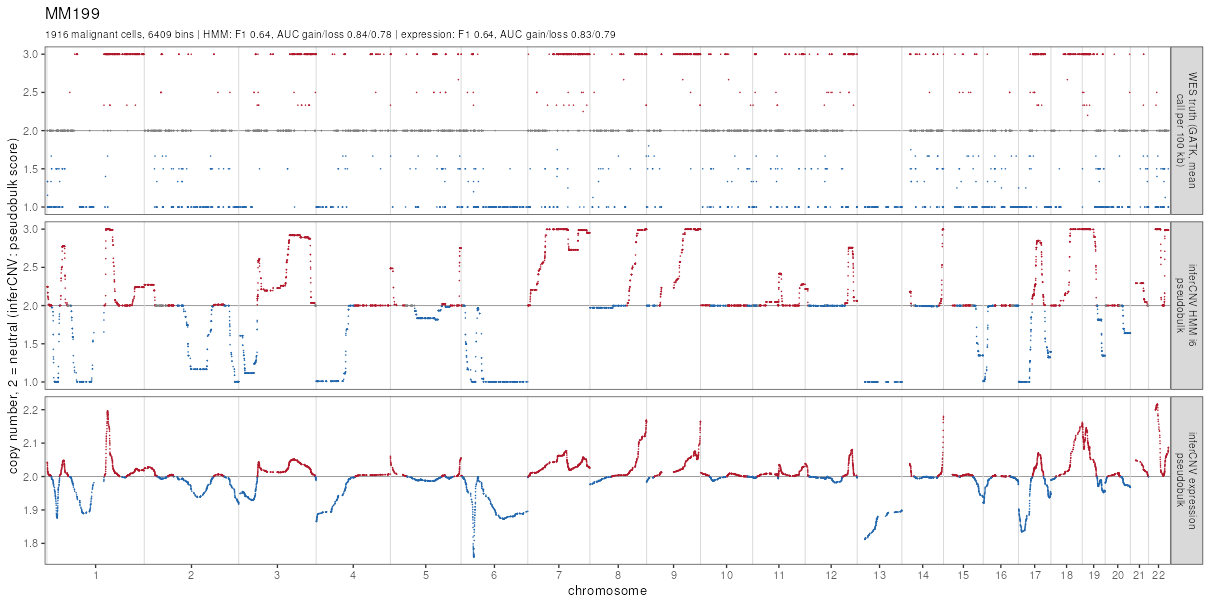
\includegraphics[width=\textwidth]{figures/fig4_MM199_genome.png}
\caption{\textbf{Comparison with DNA-based copy number in multiple myeloma MM199 (10x).} Top, whole-exome copy number segments (Schmid et al.~truth). Below, inferCNV pseudobulk scores over 1,916 malignant cells: HMM states after Bayesian filtering (CNV score) and final residual expression (expression score), in 100-kb bins along the genome. \todo{Panel with ROC curves and metric summary, if wanted; RESULT PENDING: BCH869 panel against WGS clone copy number.} Settings as in Methods.}
\label{fig:4}
\end{figure}

\begin{figure}[p]
\centering
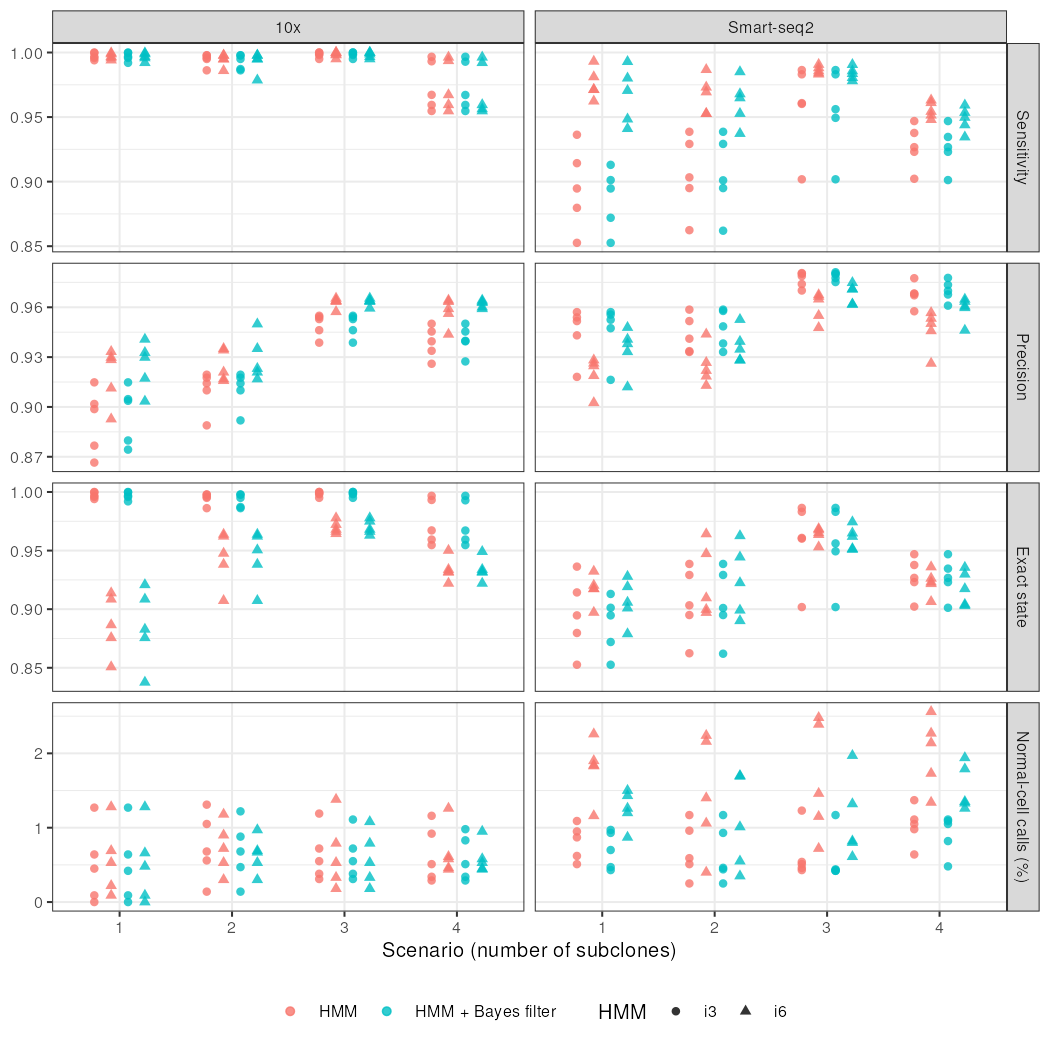
\includegraphics[width=\textwidth]{figures/fig5_simulation.png}
\caption{\textbf{Accuracy on simulated tumours.} Sensitivity, precision, exact-state accuracy, reference call rate and subcluster purity of the i6 HMM after Bayesian filtering for simulated 10x and Smart-seq2 data with one to four subclones (sim1--sim4), over five seeds (points) with means (bars); values in Table 1. \todo{Optional inset: i3 against i6.} \todo{Figure drawn from analyses/simulation/fig5\_simulation.png; check that it shows the master-build numbers of Table 1.}}
\label{fig:5}
\end{figure}

\begin{figure}[p]
\centering
\fbox{\parbox[c][4cm][c]{0.9\textwidth}{\centering Figure 6 pending}}
\caption{\textbf{Specificity and scale.} \todo{RESULT PENDING} (a) Non-neutral call rate in PBMC from healthy donors, by cell type, before and after Bayesian filtering. (b) Run time and peak memory against number of cells, with and without the Bayesian model and for i6 and i3.}
\label{fig:6}
\end{figure}

\begin{figure}[p]
\centering
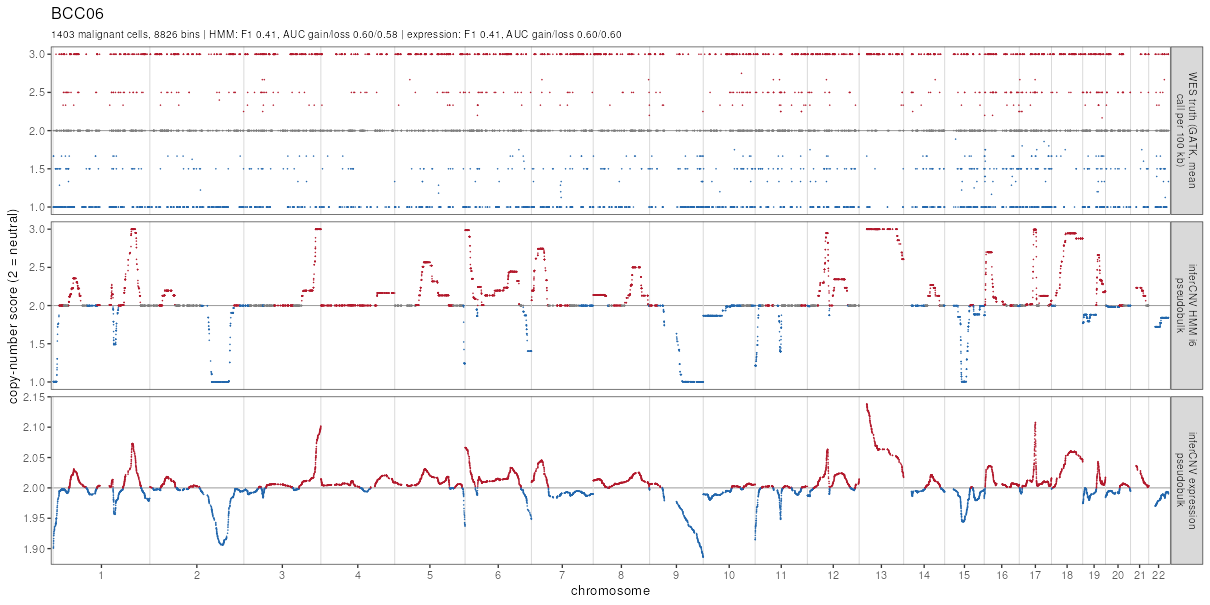
\includegraphics[width=\textwidth]{figures/figS1_BCC06_genome.png}
\caption{\textbf{Basal cell carcinoma BCC06 before and after treatment.} As Fig. 4, for BCC06 (1,403 malignant and 33 reference cells) and BCC06post (320 malignant and 280 reference cells). The exome segmentation of these samples is highly fragmented; see text.}
\label{fig:S1}
\end{figure}

% Supplementary Table S2: Metrics against DNA-based copy number.
% For each sample and score: number of malignant cells and bins, maximal F1, sensitivity and precision for gains and losses at the optimum, AUC and partial AUC for gains and losses, Pearson r; with the values reported by Schmid et al.~for inferCNV v1.10. (From analyses/fig4/metrics\_fig4.tsv and schmid2025\_reported\_infercnv\_v1.10.tsv.)


\end{document}
